\section{ChatCoT 实验}
\subsection{实验结果分析}
\begin{frame}{实验结果分析}
    \begin{enumerate}
        \item 从表中可以看到,检索增强方法(如 ChatCoT 和 CoT w/ Retri)优于其他方法。可能是因为检索到的示例可能包含更多相关的知识和推理步骤,ChatGPT 对几何领域的知识和符号相对较为陌生。如果没有类似的示例,大型语言模型很难准确理解这些内容。
        
        \pause
        \item 可以发现,直接在推理过程中使用外部工具甚至可能产生负面影响。原因可能在于,将工具使用融入 CoT 推理过程会影响推理的连贯性。
    \end{enumerate}
\end{frame}

\begin{frame}{实验结果图表}
    \begin{figure}
        \centering
        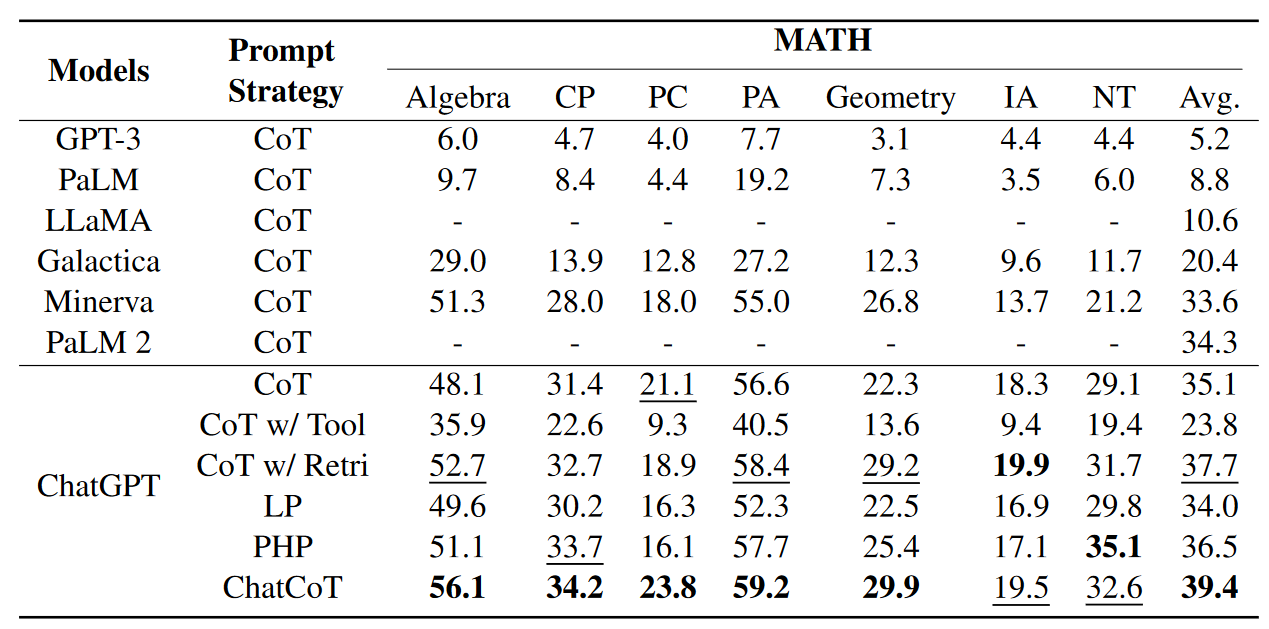
\includegraphics[width=.7\linewidth]{./pic/math.png}
        \caption{math 结果}
        \label{fig:result1}
    \end{figure}
\end{frame}
\begin{frame}{实验结果图表}
    \begin{figure}
        \centering
        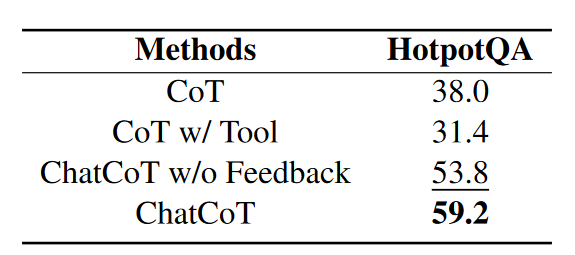
\includegraphics[width=.7\linewidth]{./pic/hotpotqa.png}
        \caption{HotpotQA 结果}
        \label{fig:result2}
    \end{figure}
\end{frame}

% Section: Prompt Design
\subsection{代码中的 prompt 设计}


\begin{frame}{Prompt 设计}
    \begin{figure}
        \centering
        
\includegraphics[width=.5\linewidth]{./pic/1.png}
        % \caption{HotpotQA 结果}
        % \label{fig:result2}
    \end{figure}
\end{frame}

% \begin{frame}{Prompt 设计}
%     \begin{verbatim}
%         EquationSolver_UnknownVariable = {
%         "role": "user",
%         "content": "Give me the unknown variable of the equation system 
%         in latex style and separated by comma"
%     },
%     EquationSolver_EquationSystem = {
%         "role": "user",
%         "content": "Give me the equation system in latex style 
%         and separated by comma"
%     },
%     Calculator_Equation = {
%         "role": "user",
%         "content": "Give me the equation to calculate in latex 
%         style and separated by comma"
%     }
%     \end{verbatim}
% \end{frame}

\begin{frame}{Prompt 示例}
    有5个这样的 prompt chat:
    \begin{figure}
        \centering
        
\includegraphics[width=.5\linewidth]{./pic/2.png}
        % \caption{HotpotQA 结果}
        % \label{fig:result2}
    \end{figure}

\end{frame}



\begin{frame}{Prompt 示例}
    \begin{figure}
        \centering
        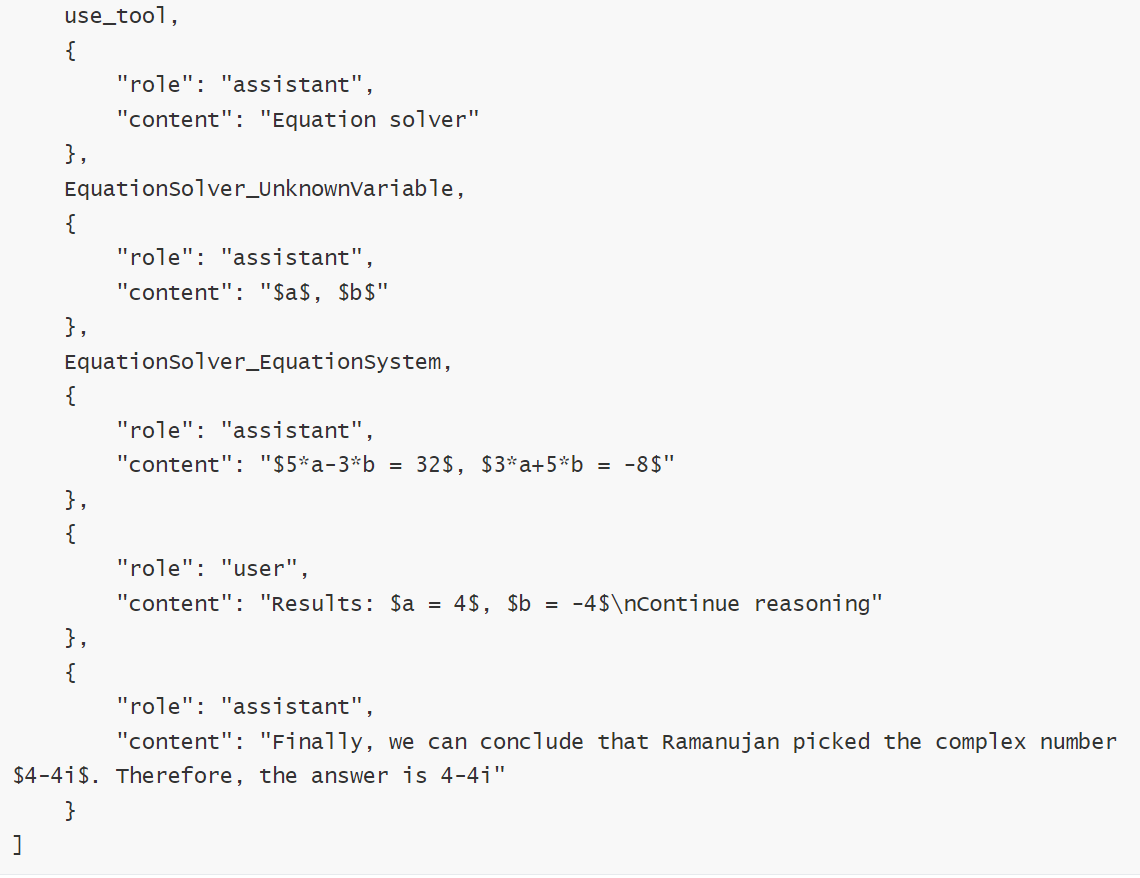
\includegraphics[width=.5\linewidth]{./pic/3.png}
        % \caption{HotpotQA 结果}
        % \label{fig:result2}
    \end{figure}
\end{frame}

\begin{frame}{Begin Prompt}
    \begin{figure}
        \centering
        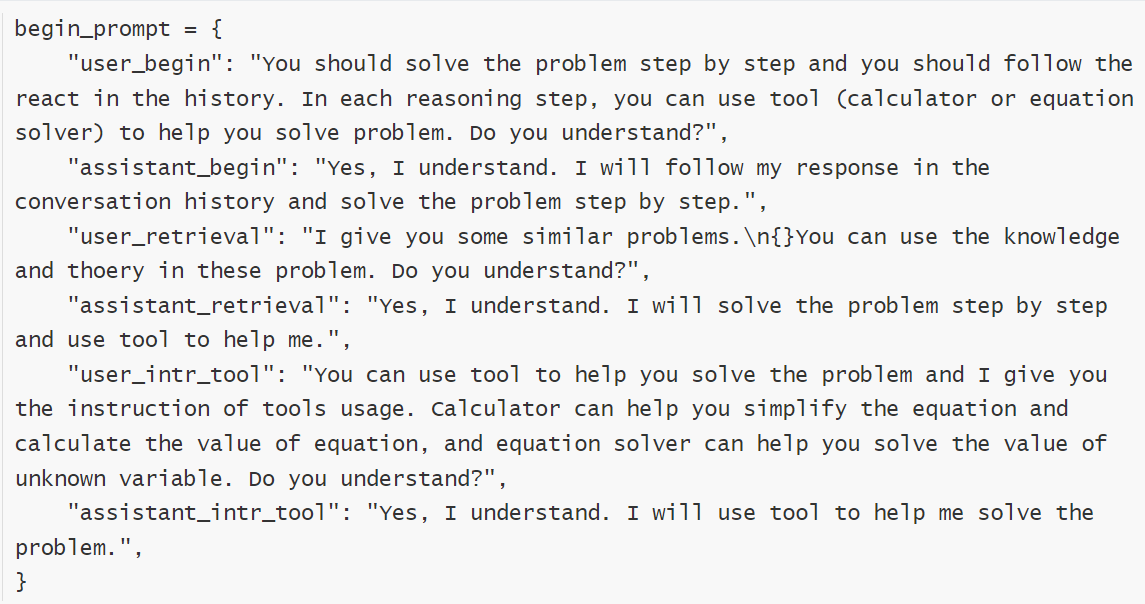
\includegraphics[width=.7\linewidth]{./pic/4.png}
        % \caption{HotpotQA 结果}
        % \label{fig:result2}
    \end{figure}
\end{frame}

% Section: Code Issues and Solutions
\subsection{源代码的问题}

\begin{frame}{源代码的问题}
    判断预测值和真实值的时候会出现本来应该判断为对,但却错误判断为错了,原因在于代码中判断正误太草率,仅仅是使用 \texttt{==},而实际上,会出现这些情况:
    % \begin{verbatim}
    % "llm_answer": "\\boxed{1.0}",
    % "real_answer": "1",
    % "score": false
    
    % "llm_answer": "\\boxed{1.0}",
    % "real_answer": "1",
    % "score": false
    
    % "llm_answer": "\\boxed{0.25}",
    % "real_answer": "\\frac{1}{4}",
    % "score": false
    % \end{verbatim}
    \begin{figure}
        \centering
        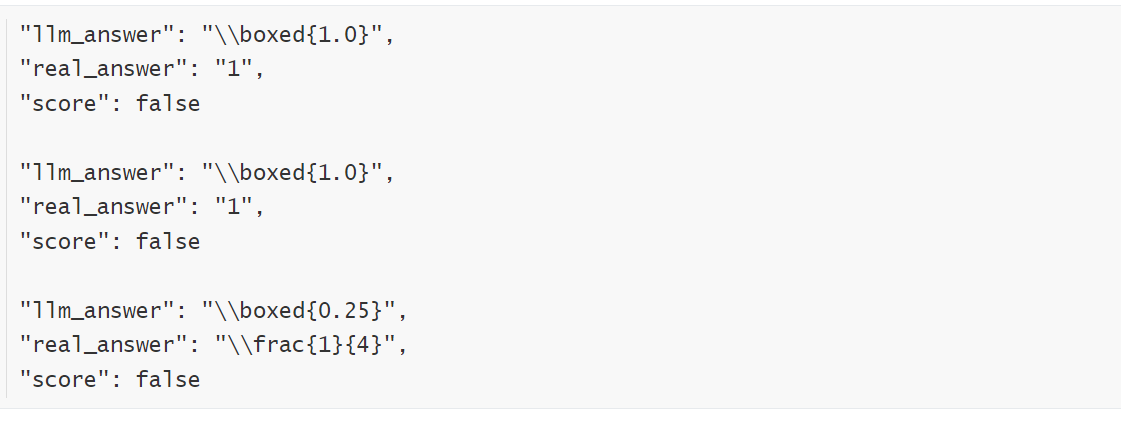
\includegraphics[width=.7\linewidth]{./pic/5.png}
        % \caption{HotpotQA 结果}
        % \label{fig:result2}
    \end{figure}
    
    这些都应该是对的。
\end{frame}

\begin{frame}{代码修改方案}
    修改为这样可以解决这种情况:
    
    % \begin{verbatim}
    % data['llm_answer'] = pred
    % data['real_answer'] = real_label
    
    % data['score'] = False
    % if isinstance(pred, str) and pred.startswith("\\boxed{") and pred.endswith("}"):
    %     pred = pred[7:-1]
    
    %     llm_value = pred
    %     real_value = real_label
    %     try:
    %         llm_value = float(pred)
    %         real_value = float(real_label)
    %     except ValueError:
    %         continue
    %     if isclose(llm_value, real_value):
    %         num_correct = num_correct + 1
    %         data['score'] = True
    % \end{verbatim}
    \begin{figure}
        \centering
        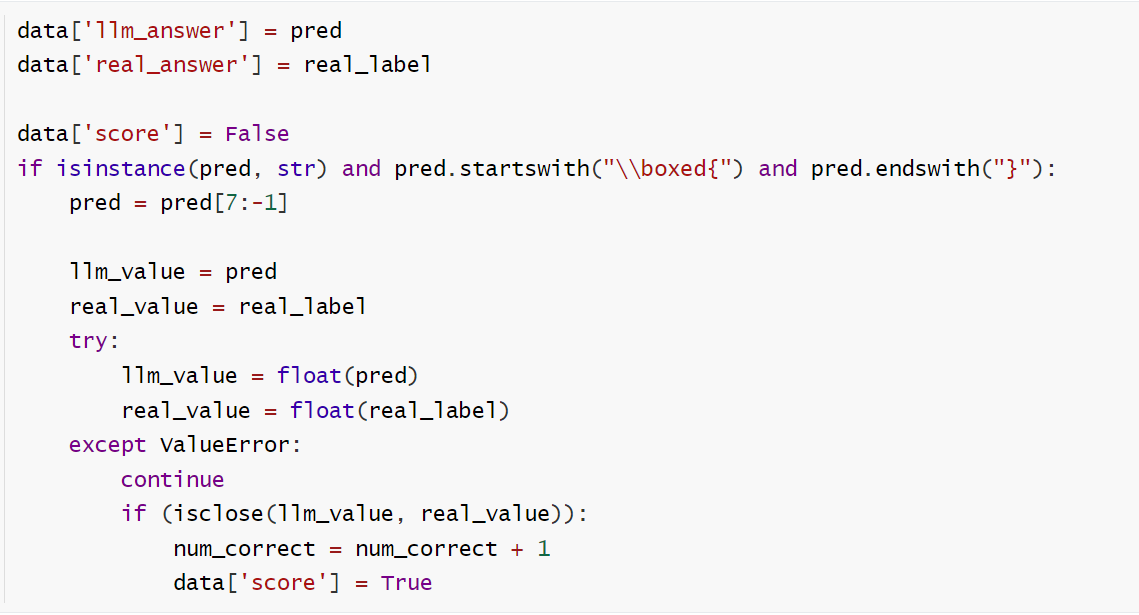
\includegraphics[width=.7\linewidth]{./pic/6.png}
        % \caption{HotpotQA 结果}
        % \label{fig:result2}
    \end{figure}
\end{frame}

% Section: Experimental Results
\subsection{实验结果}

\begin{frame}{实验结果}
    math\_algebra 一共有 1187 条数据,选择其中100条,分别选用 gpt-3.5-turbo 和 gpt-4o-2024-1120 进行测试,结果如下:
    
    \textbf{正确率}:
    \begin{itemize}
        \item gpt-3.5-turbo:  \textbf{58/101}(论文仓库中有一个完整的 output,正确率为 $348/1187 \approx 0.29$,但是论文中却说有 56.1\%,疑似造假,但也有可能是手动把那些本应该计为正确,但代码输出为 false 的算作正确了,原始结果中有很多是这种情况的,改进后没有出现这种情况)
        \item gpt-4o-2024-1120: \textbf{59/101}
    \end{itemize}
    
    一共请求 API \textbf{3855} 次;一共花费 \textbf{\$ 3.437}
    
    对于 ChatCoT 来说,gpt-4o-2024-1120 比 gpt-3.5-turbo 提升不明显。
\end{frame}
